\documentclass[11pt,a4paper]{article}

\usepackage[margin=1in]{geometry}
\usepackage{graphicx}
\usepackage{booktabs}
\usepackage{tabularx}
\usepackage{hyperref}
\usepackage{listings}
\usepackage{xcolor}
\usepackage{enumitem}
\usepackage{float}
\usepackage{fancyhdr}
\usepackage{titlesec}
\usepackage[T1]{fontenc}
\usepackage{lmodern}
\usepackage{parskip}

\hypersetup{
    colorlinks=true,
    linkcolor=blue!70!black,
    urlcolor=blue!70!black,
    citecolor=blue!70!black,
}

\lstset{
    basicstyle=\ttfamily\small,
    breaklines=true,
    frame=single,
    backgroundcolor=\color{gray!8},
    rulecolor=\color{gray!40},
    xleftmargin=4pt,
    xrightmargin=4pt,
    framexleftmargin=2pt,
    columns=fullflexible,
}

\pagestyle{fancy}
\fancyhf{}
\rhead{Team 5 --- AAMSIR}
\lhead{S26CS6.401 --- Software Engineering}
\cfoot{\thepage}

\titleformat{\section}{\Large\bfseries}{}{0em}{}
\titleformat{\subsection}{\large\bfseries}{}{0em}{}
\titleformat{\subsubsection}{\normalsize\bfseries}{}{0em}{}

\begin{document}

% ============================================================================
% TITLE PAGE
% ============================================================================
\begin{titlepage}
\centering
\vspace*{2cm}
{\Huge\bfseries AAMSIR Technical Report\par}
\vspace{0.8cm}
{\Large Adaptive Architecture for Multi-Strategy\\Information Retrieval\par}
\vspace{1.5cm}
{\large Team 5 | S26CS6.401 --- Software Engineering | Project 3\par}
\vspace{2cm}

\begin{tabular}{ll}
\toprule
\textbf{Team Member} & \textbf{Roll Number} \\
\midrule
Arihant Tripathy & 2023111026 \\
Aviral Gupta & 2023111023 \\
Inesh Dheer & 2023111010 \\
Mohit Kumar Singh & 2023111021 \\
Sreemaee Akshathala & 2025701028 \\
\bottomrule
\end{tabular}

\vspace{2cm}
{\large GitHub Repository:\par}
\url{https://github.com/Arihant25/aamsir}

\vfill
{\large April 2026\par}
\end{titlepage}

% ============================================================================
% TABLE OF CONTENTS
% ============================================================================
\tableofcontents
\newpage

% ============================================================================
% 1. INTRODUCTION
% ============================================================================
\section{Introduction}

\subsection{Problem Statement}

Institutions accumulate large volumes of internal documents --- policies, SOPs, guidelines, and knowledge bases --- that employees frequently need to query. Existing solutions are either too shallow (keyword search misses semantically related content) or privacy-compromising (cloud-hosted LLMs require sensitive documents to leave the organization's network).

\subsection{Solution: AAMSIR}

AAMSIR (Adaptive Architecture for Multi-Strategy Information Retrieval) addresses this gap with a chatbot-style interface backed by three interchangeable retrieval strategies --- syntactic, semantic, and agentic --- all running on compact, on-premise models to preserve institutional privacy.

\subsection{Technology Stack}

\begin{table}[H]
\centering
\begin{tabular}{ll}
\toprule
\textbf{Layer} & \textbf{Technology} \\
\midrule
Backend & Python 3.11+, FastAPI, uv (package manager) \\
Vector Database & ChromaDB (embedded, on-premise) \\
Relational Database & SQLite (via SQLAlchemy) \\
Embeddings & sentence-transformers (all-MiniLM-L6-v2) \\
Keyword Search & rank\_bm25 \\
LLM (Optional) & Ollama (qwen2.5:7b) \\
Frontend & Next.js 16, TypeScript, Tailwind CSS \\
PDF Extraction & pdfplumber \\
\bottomrule
\end{tabular}
\caption{Technology Stack}
\end{table}


% ============================================================================
% 2. TASK 1: REQUIREMENTS AND SUBSYSTEMS
% ============================================================================
\section{Task 1: Requirements and Subsystems}

\subsection{Functional Requirements}

\begin{table}[H]
\centering
\small
\begin{tabularx}{\textwidth}{llX}
\toprule
\textbf{ID} & \textbf{Requirement} & \textbf{Architectural Significance} \\
\midrule
FR-01 & Query Interface Dashboard & Drives the Facade pattern (single API entry point) \\
FR-02 & Result Exploration & Requires chunked storage, metadata tracking, and file-serving endpoint \\
FR-03 & User Feedback Module & Requires persistence layer and analytics \\
FR-04 & Multi-Modal Retrieval & Drives Strategy Pattern and Microkernel \\
FR-05 & Retrieval Configuration Panel & Drives runtime strategy switching \\
FR-06 & Document Management Module & Drives Pipe-and-Filter ingestion pipeline \\
FR-07 & Conversational Query Refinement & Drives two-phase LLM invocation: rewrite $\to$ retrieve $\to$ generate \\
\bottomrule
\end{tabularx}
\caption{Functional Requirements}
\end{table}

\subsection{Non-Functional Requirements}

\begin{table}[H]
\centering
\begin{tabular}{lll}
\toprule
\textbf{ID} & \textbf{Requirement} & \textbf{Target} \\
\midrule
NFR-01 & Latency & P95 $\leq$ 15 seconds \\
NFR-02 & Throughput & $\geq$ 50 concurrent users \\
NFR-03 & Scalability & 10,000 indexed documents \\
NFR-04 & Availability & $\geq$ 99\% during working hours \\
NFR-05 & Modifiability & New strategies in $<$ 100 person-hours \\
NFR-06 & Data Security & 100\% on-premise, AES-256 at rest \\
\bottomrule
\end{tabular}
\caption{Non-Functional Requirements}
\end{table}

\subsection{Architecturally Significant Requirements}

\begin{itemize}
    \item \textbf{ASR-01 (Extensibility):} Drove adoption of Microkernel + Strategy Pattern. The NLP field evolves rapidly; new retrieval methods must be addable without rewriting the core system.
    \item \textbf{ASR-02 (Latency via Context Limitation):} Drove Chain of Responsibility in semantic retrieval. SLMs have finite context windows; feeding all retrieved documents would violate latency constraints.
    \item \textbf{ASR-03 (Scalability of Ingestion):} Drove Pipe-and-Filter architecture. Processing 10,000 documents involves heavy compute steps that can bottleneck the system.
    \item \textbf{ASR-04 (Fault Tolerance):} Drove plugin sandboxing in the Microkernel. Agentic retrieval involves complex tool execution which may hang or fail.
\end{itemize}

\subsection{Subsystem Overview}

The system is divided into five subsystems:

\begin{enumerate}
    \item \textbf{Presentation Layer:} Next.js web dashboard with query interface, document management, and settings.
    \item \textbf{Document Ingestion Pipeline:} Pipe-and-Filter architecture for Extract $\to$ Summarize $\to$ Chunk $\to$ Embed $\to$ Index.
    \item \textbf{Hybrid Retrieval Engine:} Microkernel with Syntactic, Semantic, and Agentic strategy plugins.
    \item \textbf{Generation \& Orchestration Layer:} Orchestrator (Facade), Context Aggregator (RRF), answer generation.
    \item \textbf{Data Persistence Layer:} SQLite for metadata/feedback, ChromaDB for vector embeddings.
\end{enumerate}

\begin{figure}[H]
\centering
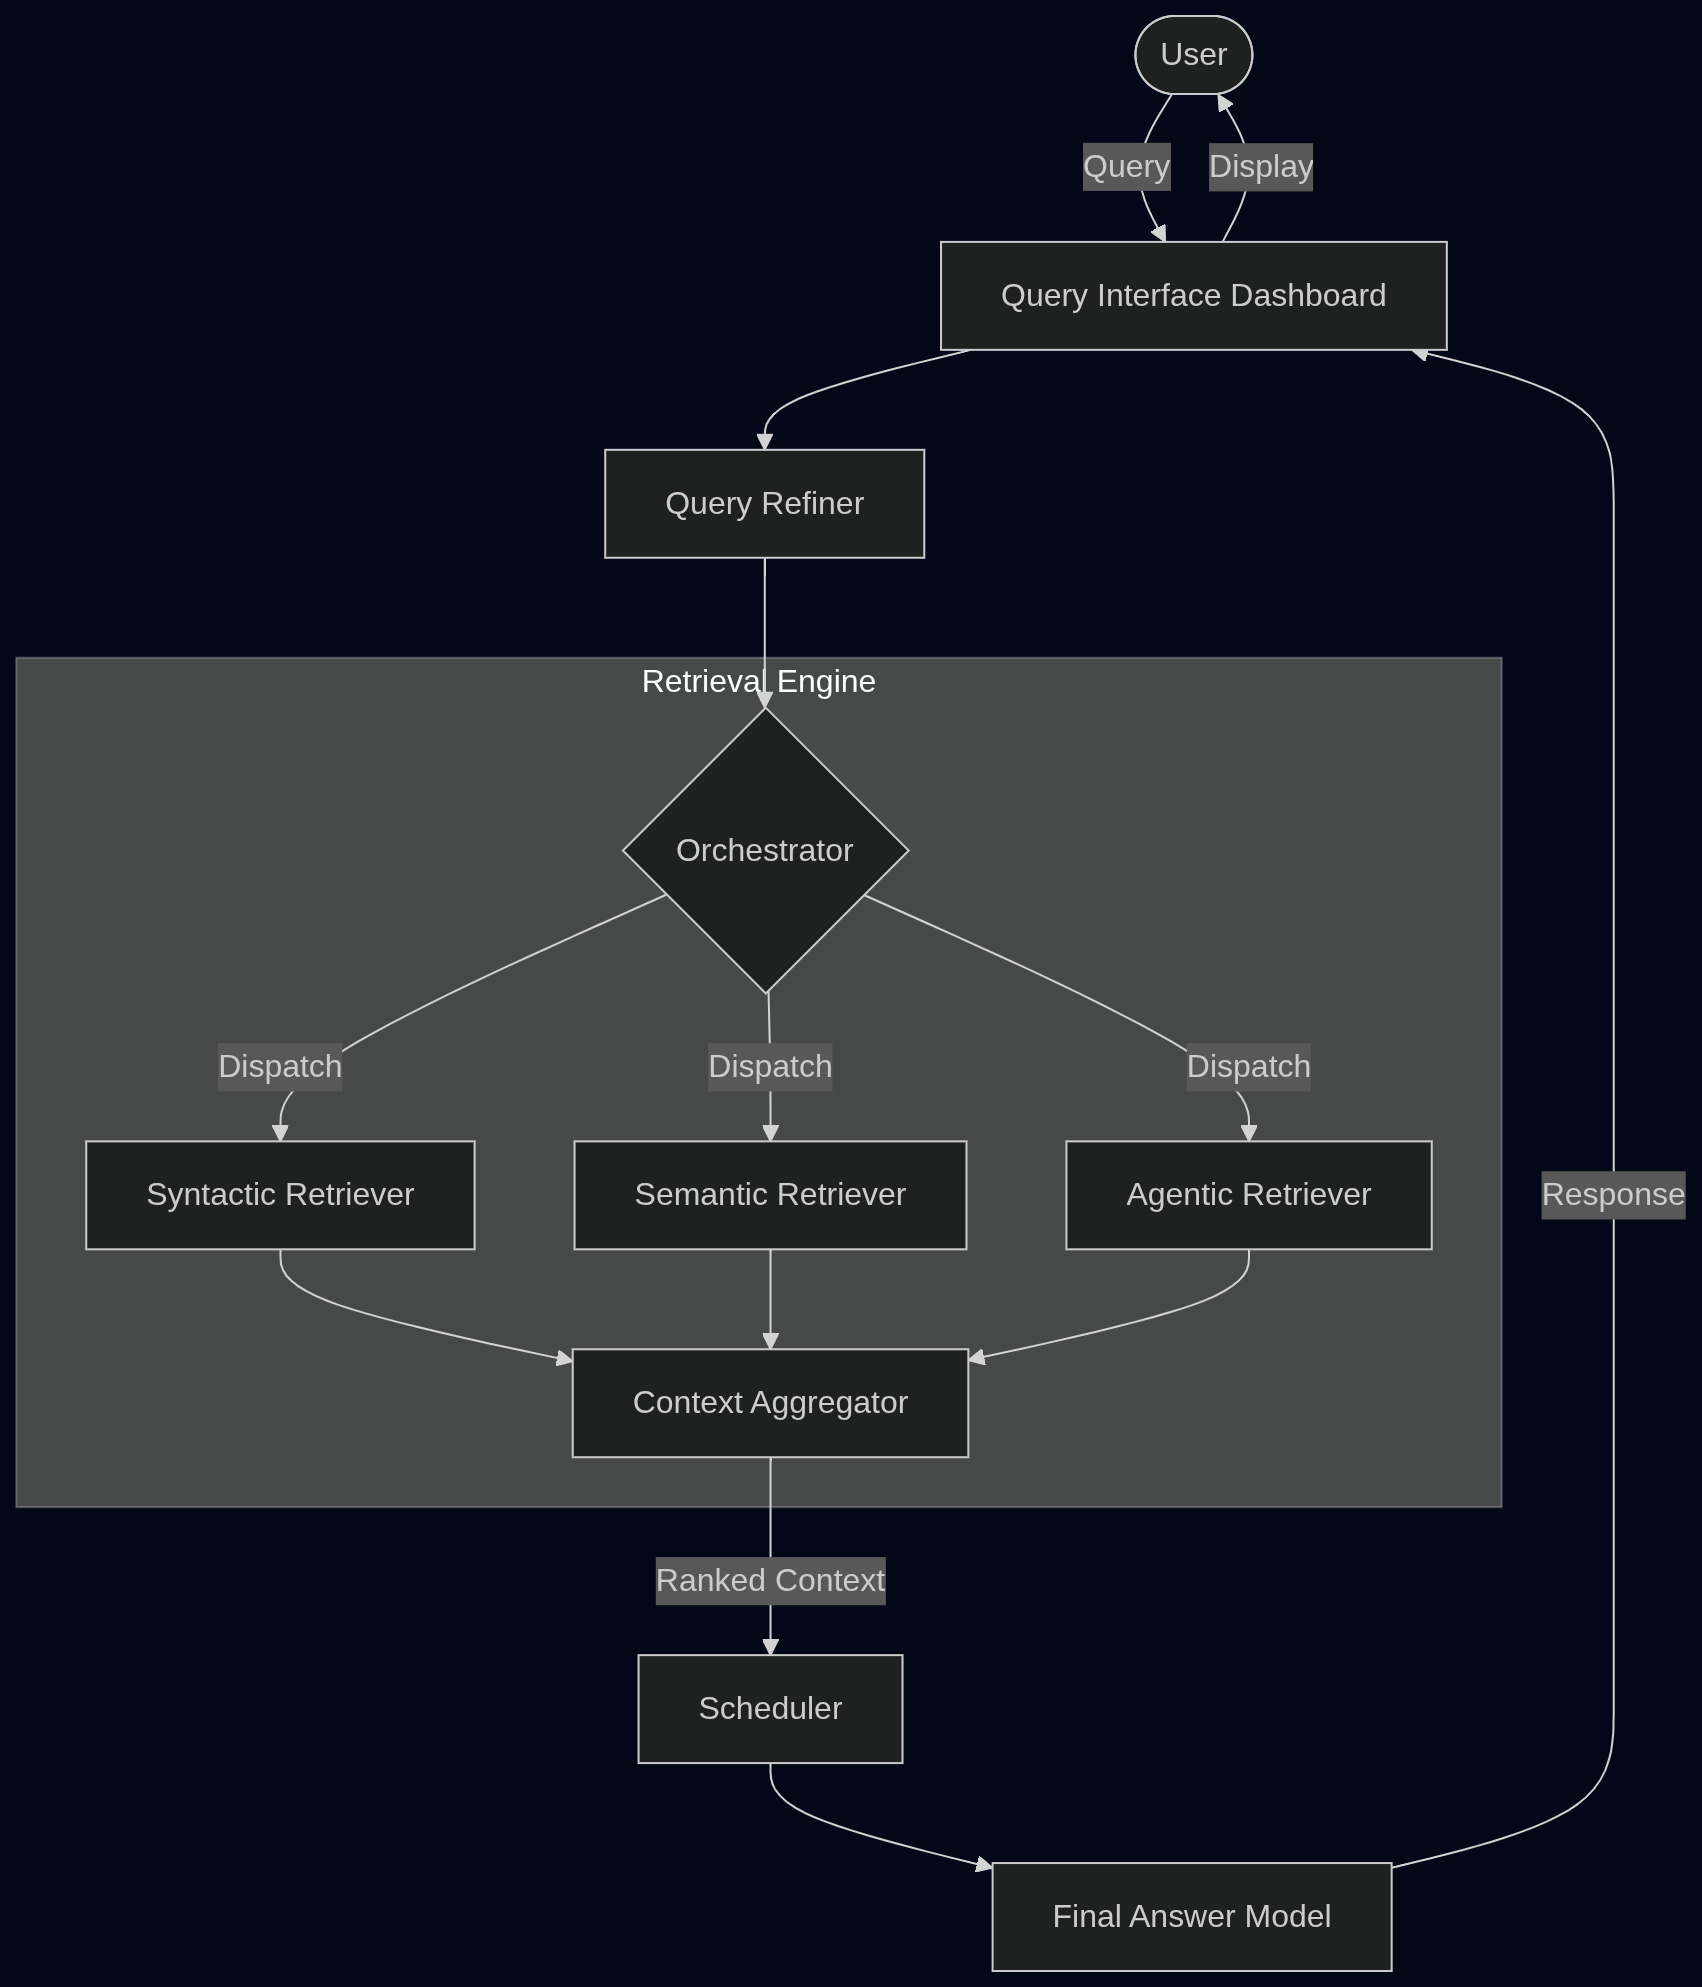
\includegraphics[width=0.65\textwidth]{Task1/archView.png}
\caption{High-level architecture showing the flow of a user query through the Presentation, Retrieval Engine, and Generation layers.}
\label{fig:archview}
\end{figure}

\begin{figure}[H]
\centering
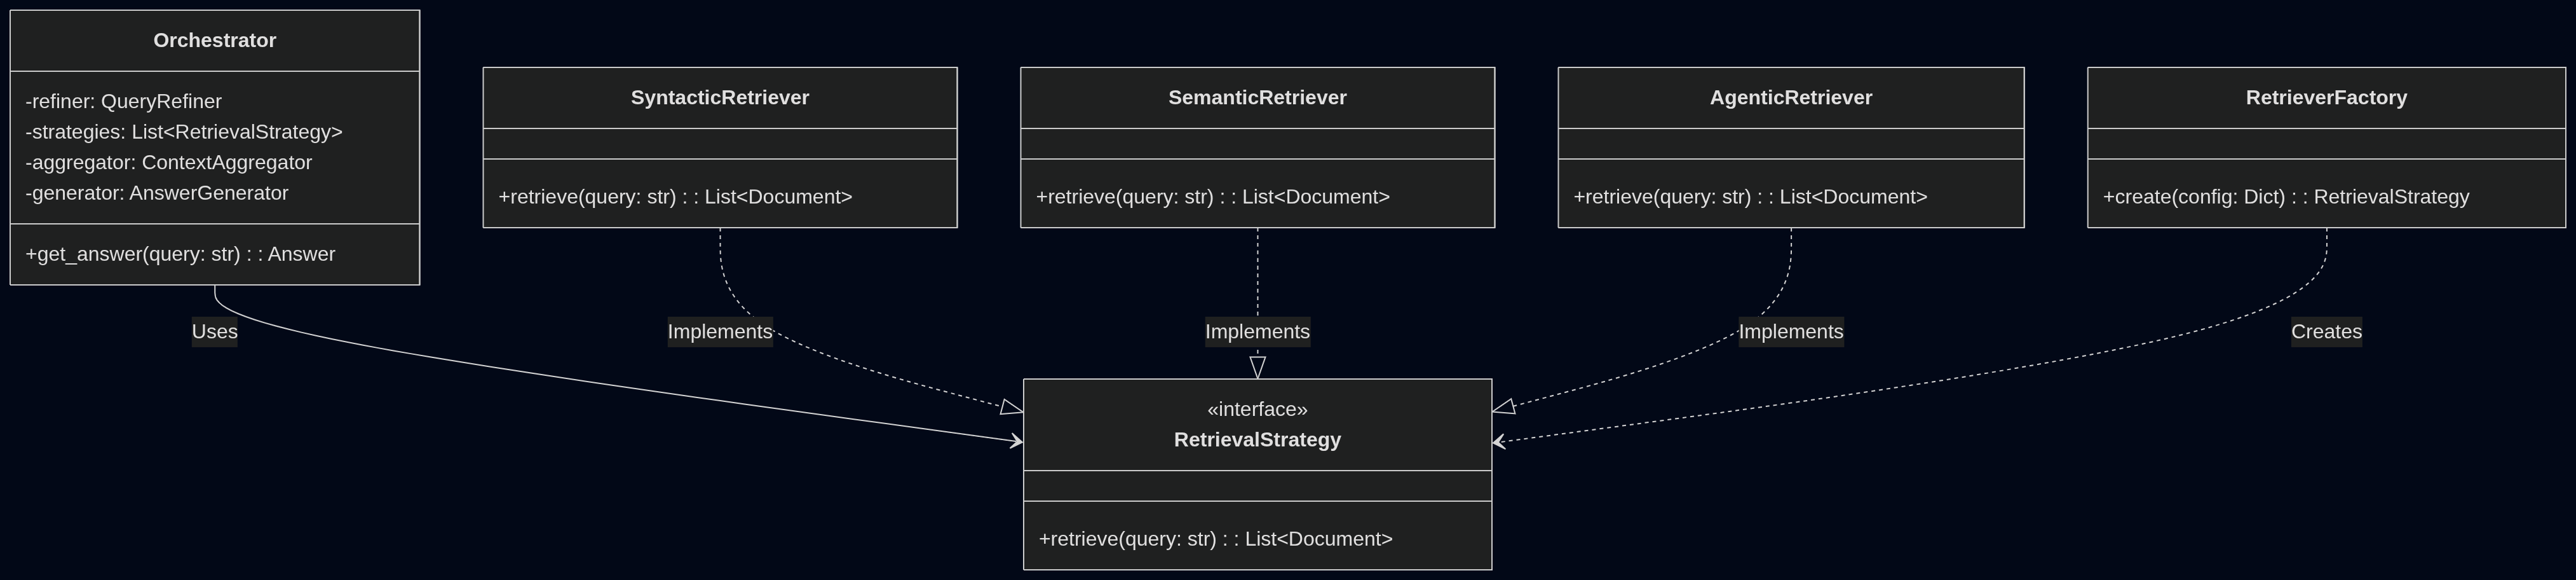
\includegraphics[width=\textwidth]{Task1/classDiagram.png}
\caption{UML class diagram of the retrieval engine: Orchestrator (Facade), RetrievalStrategy (interface), concrete retrievers, and RetrieverFactory.}
\label{fig:classdiagram}
\end{figure}


% ============================================================================
% 3. TASK 2: ARCHITECTURE FRAMEWORK
% ============================================================================
\section{Task 2: Architecture Framework}

\subsection{Stakeholder Identification (IEEE 42010)}

\begin{table}[H]
\centering
\small
\begin{tabularx}{\textwidth}{lX}
\toprule
\textbf{Stakeholder} & \textbf{Concerns} \\
\midrule
End Users (Researchers/Students) & Precision, Latency, Usability, Trustworthiness \\
System Administrators & Deployability, Availability, Resource Efficiency, Observability \\
Course Instructors/Evaluators & Compliance to Standards, Modularity, Design Pattern Correctness \\
Developers/Maintenance Team & Modifiability, Testability, Maintainability \\
Data Owners/Content Providers & Data Integrity, Confidentiality \\
\bottomrule
\end{tabularx}
\caption{Stakeholders and Concerns (IEEE 42010)}
\end{table}

\subsubsection{Viewpoints and Views}

Four viewpoints are used to address stakeholder concerns:

\begin{enumerate}
    \item \textbf{Functional / Logical Viewpoint:} Describes what the system does --- the Orchestrator facade, strategy plugins, and context aggregation logic. Addressed via UML class and sequence diagrams.
    \item \textbf{Development / Module Viewpoint:} Describes the package decomposition (\texttt{api/}, \texttt{ingestion/}, \texttt{retrieval/}, \texttt{database.py}, \texttt{config.py}). Each plugin depends only on the \texttt{RetrievalStrategy} interface.
    \item \textbf{Deployment / Operational Viewpoint:} All components run on-premise: Next.js frontend, FastAPI backend, SQLite, ChromaDB, and Ollama within the institution's network boundary.
    \item \textbf{Information / Data Viewpoint:} Documents transition through three representations: raw upload (filesystem), structured record (SQLite), and vector index (ChromaDB).
\end{enumerate}

\subsection{Architecture Decision Records (ADRs)}

All ADRs follow the Nygard template (Status, Context, Decision Drivers, Considered Options, Decision Outcome, Pros/Cons).

\subsubsection{ADR-001: Microkernel for Retrieval Engine}
\begin{itemize}[leftmargin=*]
    \item \textbf{Context:} Multiple evolving retrieval strategies require independent addition/removal.
    \item \textbf{Decision:} Adopt Microkernel (Plugin) Architecture.
    \item \textbf{Consequences:} Open/Closed Principle satisfied; fault isolation; simplified testing.
    \item \textbf{Alternatives Rejected:} Monolithic Controller (violates OCP), Microservices (excessive overhead).
\end{itemize}

\subsubsection{ADR-002: Pipe-and-Filter for Ingestion}
\begin{itemize}[leftmargin=*]
    \item \textbf{Context:} Document ingestion involves fixed-order transformations that need flexible step swapping.
    \item \textbf{Decision:} Implement Pipe-and-Filter Architecture.
    \item \textbf{Consequences:} Loose coupling, supports parallelism, maintainability.
    \item \textbf{Alternatives Rejected:} Batch Script (monolithic failure), Event-Driven (excessive complexity).
\end{itemize}

\subsubsection{ADR-003: Strategy Pattern for Retrieval Algorithms}
\begin{itemize}[leftmargin=*]
    \item \textbf{Context:} Three different retrieval algorithms need runtime interchangeability.
    \item \textbf{Decision:} Implement Strategy Pattern with \texttt{RetrievalStrategy} interface.
    \item \textbf{Consequences:} Clean separation, independently testable, OCP compliance.
    \item \textbf{Alternatives Rejected:} Conditional Logic (violates OCP), Template Method (algorithms differ too much).
\end{itemize}

\subsubsection{ADR-004: Broker Pattern with Scheduler}
\begin{itemize}[leftmargin=*]
    \item \textbf{Context:} Multiple concurrent requests competing for limited GPU resources.
    \item \textbf{Decision:} Implement Broker Pattern with task queue and worker pool.
    \item \textbf{Consequences:} Asynchronous processing, load management, resilience.
    \item \textbf{Alternatives Rejected:} Direct Sync Calls (blocking), Observer Pattern (inefficient load balancing).
\end{itemize}


% ============================================================================
% 4. TASK 3: ARCHITECTURAL TACTICS AND PATTERNS
% ============================================================================
\section{Task 3: Architectural Tactics and Patterns}

\subsection{Architectural Tactics}

\begin{table}[H]
\centering
\small
\begin{tabularx}{\textwidth}{clcX}
\toprule
\textbf{\#} & \textbf{Tactic} & \textbf{Category} & \textbf{NFR Addressed} \\
\midrule
1 & Caching Proxy & Performance & NFR-01 (Latency $\leq$ 15s P95) \\
2 & Cascading / Progressive Narrowing & Performance & NFR-01 (Latency $\leq$ 15s P95) \\
3 & Fault Isolation via Plugin Sandboxing & Availability & NFR-04 (Uptime $\geq$ 99\%) \\
4 & Horizontal Scaling of Stateless Filters & Scalability & NFR-03 (10K documents) \\
5 & Task Queuing with Resource Pooling & Throughput & NFR-02 (50 concurrent users) \\
\bottomrule
\end{tabularx}
\caption{Architectural Tactics}
\end{table}

\textbf{Tactic 1 --- Caching (Proxy):} The \texttt{CachingAgenticProxy} wraps the expensive \texttt{AgenticRetriever} with an LRU cache (128 entries, MD5-keyed). Cache hits return in $<$1ms instead of the 5--30s agentic retrieval time.

\textbf{Tactic 2 --- Cascading / Progressive Narrowing:} The \texttt{SemanticRetriever} implements a Chain of Responsibility pipeline with three stages: TitleMatch (very low cost), SummarySim (low cost), ContentSim (medium cost). This reduces full-content vector comparisons from $\sim$10,000 to $\sim$75, a 99.25\% reduction.

\textbf{Tactic 3 --- Fault Isolation:} The Orchestrator wraps each plugin invocation in an exception boundary. If a plugin crashes or times out, the kernel logs the failure and returns partial results from healthy plugins.

\textbf{Tactic 4 --- Horizontal Scaling:} The ingestion pipeline's stateless filters can be replicated across multiple workers. The Embedder filter (most compute-intensive) can scale to N workers consuming from a shared queue.

\textbf{Tactic 5 --- Task Queuing with Resource Pooling:} The Scheduler component acts as a Broker between the Orchestrator and model inference workers, buffering requests in a FIFO queue to smooth traffic spikes.

\subsection{Implementation Patterns}

\subsubsection{Pattern 1: Strategy Pattern}

The Strategy Pattern defines a common \texttt{RetrievalStrategy} interface for a family of retrieval algorithms. Concrete strategy classes (\texttt{SyntacticRetriever}, \texttt{SemanticRetriever}, \texttt{CachingAgenticProxy}) implement the interface. The \texttt{Orchestrator} holds a collection of strategy objects and delegates retrieval to them without any type checks or conditionals.

\textbf{How it works:}
\begin{enumerate}
    \item At startup, concrete strategies are created via \texttt{StrategyFactory.create()} and registered with the Orchestrator.
    \item When \texttt{query(query\_text)} is called, the Orchestrator iterates over its strategies list and calls \texttt{retrieve(query)} on each.
    \item Results are passed to the \texttt{ContextAggregator}, which deduplicates and re-ranks them using Reciprocal Rank Fusion.
    \item Adding a new strategy requires only implementing \texttt{RetrievalStrategy} and adding a factory case. The Orchestrator code is \emph{not modified}.
\end{enumerate}

\textbf{Consequences:} New retrieval strategies can be added without modifying the Orchestrator (OCP). Each strategy is independently unit-testable. Strategies can be enabled/disabled at runtime via the configuration panel.

\begin{figure}[H]
\centering
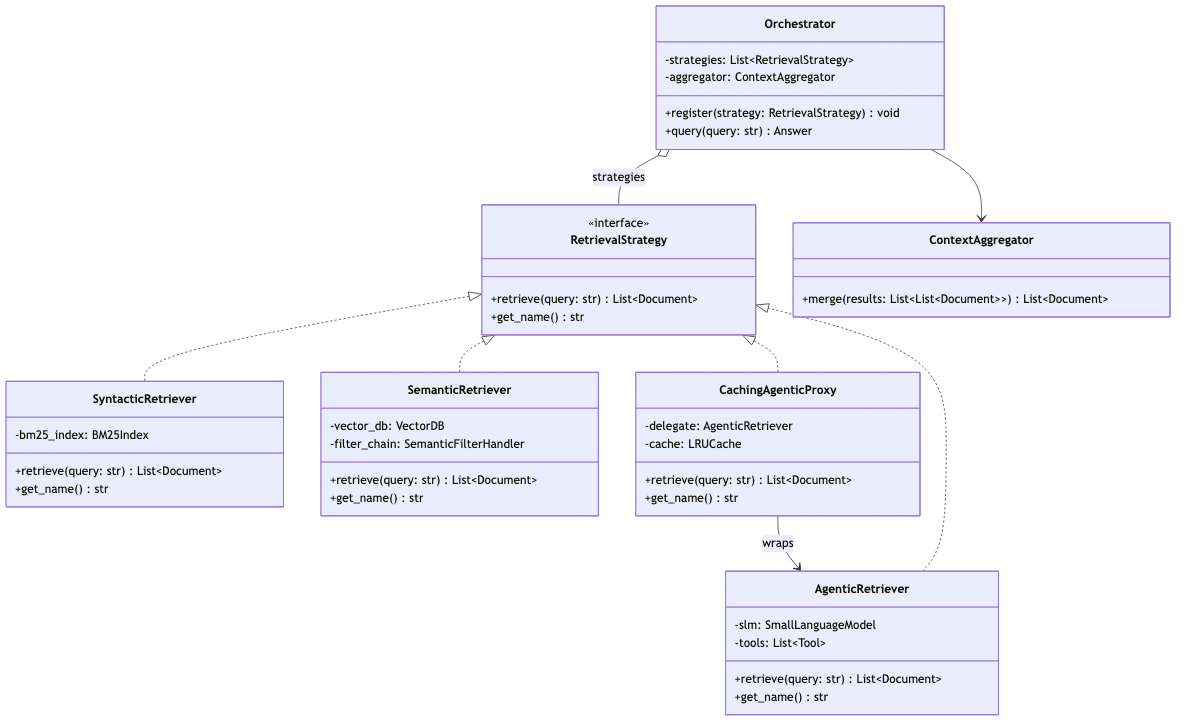
\includegraphics[width=\textwidth]{Task3/strategy_class_diagram.png}
\caption{Strategy Pattern --- Class Diagram}
\end{figure}

\begin{figure}[H]
\centering
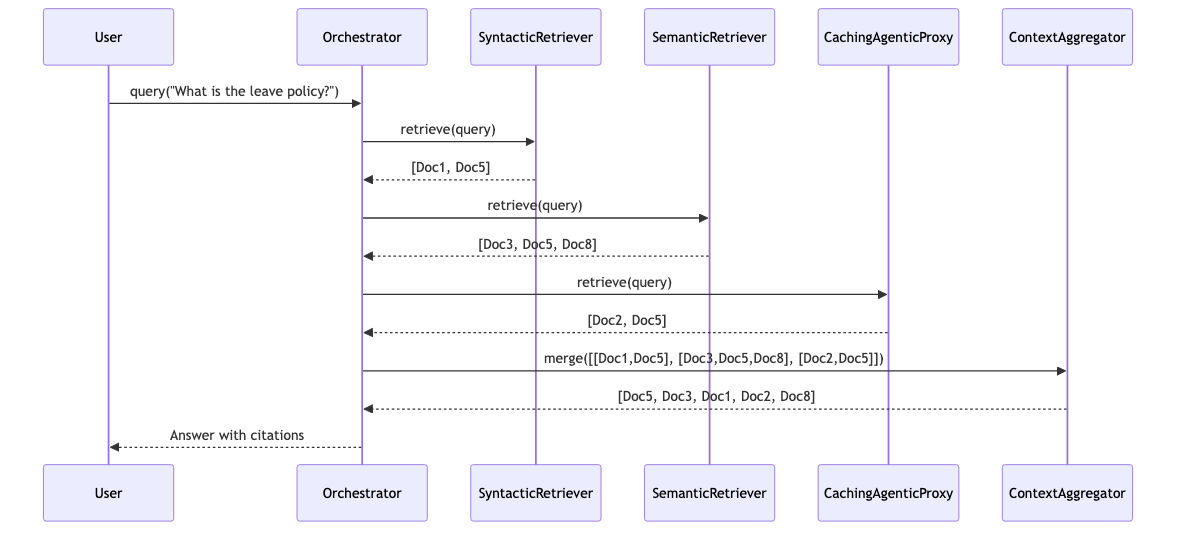
\includegraphics[width=\textwidth]{Task3/strategy_sequence_diagram.png}
\caption{Strategy Pattern --- Sequence Diagram (sequential invocation)}
\end{figure}

\subsubsection{Pattern 2: Chain of Responsibility}

The Chain of Responsibility implements a graduated filtering pipeline within the \texttt{SemanticRetriever}. An abstract \texttt{SemanticFilterHandler} defines the chain interface.

\textbf{Chain structure:}
\begin{enumerate}
    \item \texttt{TitleMatchHandler} --- Lexical overlap between query tokens and document titles. Input: $\sim$10,000 docs $\to$ Output: $\sim$800 docs. Cost: Very Low.
    \item \texttt{SummarySimHandler} --- Cosine similarity on pre-computed summary embeddings. Input: $\sim$800 docs $\to$ Output: $\sim$75 docs. Cost: Low.
    \item \texttt{ContentSimHandler} --- Full vector search via ChromaDB on filtered candidates. Input: $\sim$75 docs $\to$ Output: $\sim$15 docs. Cost: Medium.
\end{enumerate}

\textbf{Consequences:} Dramatically reduces latency of semantic search (99\%+ reduction in expensive comparisons). Each handler can be independently tuned. New filtering stages can be inserted anywhere in the chain.

\begin{figure}[H]
\centering
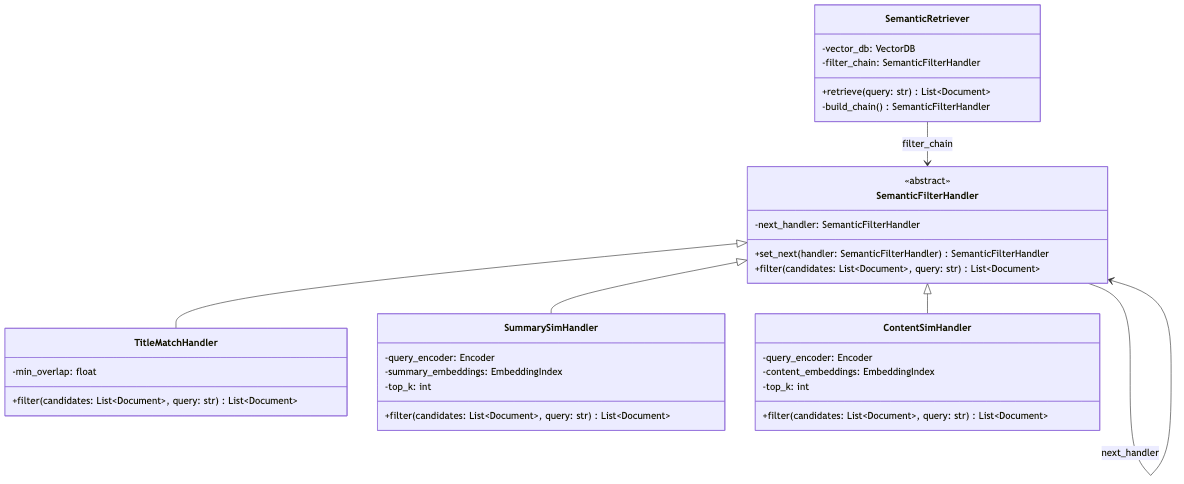
\includegraphics[width=\textwidth]{Task3/cor_class_diagram.png}
\caption{Chain of Responsibility --- Class Diagram}
\end{figure}

\begin{figure}[H]
\centering
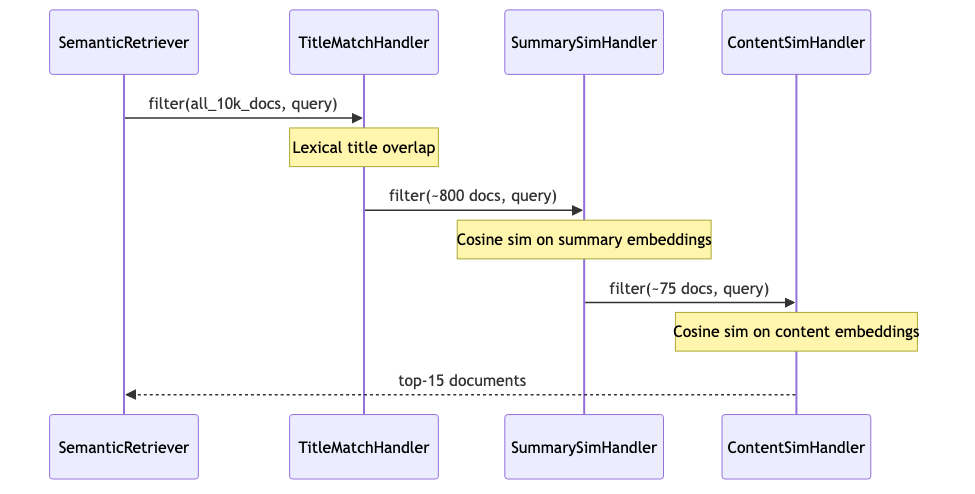
\includegraphics[width=0.9\textwidth]{Task3/cor_sequence_diagram.png}
\caption{Chain of Responsibility --- Sequence Diagram}
\end{figure}


% ============================================================================
% 5. TASK 4: PROTOTYPE IMPLEMENTATION AND ANALYSIS
% ============================================================================
\section{Task 4: Prototype Implementation and Analysis}

\subsection{Prototype Overview}

The prototype implements a \textbf{complete end-to-end query-answer pipeline}:

\begin{enumerate}
    \item User uploads documents via the web dashboard.
    \item Documents are ingested through the Pipe-and-Filter pipeline (Extract $\to$ Summarize $\to$ Chunk $\to$ Embed $\to$ Index).
    \item User submits natural-language queries.
    \item The Orchestrator invokes selected retrieval strategies sequentially with fault isolation.
    \item Results are merged using Reciprocal Rank Fusion (RRF).
    \item An answer is generated (LLM if Ollama available, extractive otherwise).
    \item Sources with citations are displayed.
    \item User can provide feedback (helpful/not helpful).
\end{enumerate}

\subsection{Key Implementation Details}

\subsubsection{Document Ingestion (Pipe-and-Filter + Adapter)}

The ingestion pipeline implements ADR-002 as five stateless filter functions operating on a \texttt{DocumentEnvelope}:

\begin{lstlisting}
extract_text() -> summarize() -> chunk_text() -> embed_chunks() -> index_document()
\end{lstlisting}

The text extraction filter uses the \textbf{Adapter Pattern} (\texttt{ExtractorRegistry}) to dynamically select the correct format handler at runtime. Adding support for a new format (e.g., \texttt{.docx}) requires only implementing the \texttt{TextExtractor} interface and registering it --- no pipeline code changes.

\subsubsection{Retrieval Engine (Microkernel + Strategy)}

The \texttt{Orchestrator} manages three retrieval plugins registered via \texttt{StrategyFactory}:

\begin{itemize}
    \item \textbf{SyntacticRetriever:} Rebuilds a BM25 index over paragraph-level chunks at query time. Applies a 50\%-of-top-score threshold to filter noise. Average latency: $\sim$2ms.
    \item \textbf{SemanticRetriever:} Adaptive --- for corpora under 100 documents it queries ChromaDB directly with a 60\%-similarity cutoff; for larger corpora it engages the full Chain of Responsibility pipeline, reducing candidate sets by $\sim$99\%. Average steady-state latency: $\sim$72ms.
    \item \textbf{CachingAgenticProxy:} Wraps \texttt{AgenticRetriever} (Ollama \texttt{qwen2.5:7b}) with an LRU cache (128 entries, MD5-keyed). Cache hits return in $<$1ms. The agentic retriever uses Ollama tool-calling to explore the document corpus across multiple inference rounds.
\end{itemize}

Each plugin is invoked inside an exception boundary (Tactic 3). If a plugin crashes or times out, the Orchestrator logs the failure and returns partial results from healthy plugins.

\subsubsection{Context Aggregation and Enrichment}

The \texttt{ContextAggregator} merges results from all active strategies using \textbf{Reciprocal Rank Fusion (RRF)} with constant $k=60$. Each document's aggregated score is:

\[
\text{score}(d) = \sum_{s \in \text{strategies}} \frac{1}{k + \text{rank}_s(d)}
\]

After merging, a relevance filter retains only chunks scoring $\geq$70\% of the top RRF score. For each relevant chunk, full document content (up to 2,000 chars) is fetched from SQLite for richer context.

\subsubsection{Conversational RAG with Query Rewriting (FR-07)}

The Orchestrator implements a two-phase LLM pipeline when conversation history is present:

\begin{enumerate}
    \item \textbf{Rewrite:} The LLM rewrites the follow-up question into a standalone search query using the last 6 messages of history.
    \item \textbf{Retrieve:} Retrieval runs using the rewritten query (BM25 + vector).
    \item \textbf{Generate:} Answer generation uses the original query + history + retrieved context.
\end{enumerate}

The rewrite step is skipped for first messages (no history), adding zero overhead. The streaming endpoint (\texttt{POST /api/query/stream}) emits four SSE event types: \texttt{rewrite}, \texttt{sources}, \texttt{token}, \texttt{done}. This phased streaming lets the frontend render cited sources immediately while the answer is still generating.

\subsubsection{Frontend}

The Next.js frontend provides three pages:
\begin{itemize}
    \item \textbf{Query Dashboard:} Streaming chatbot interface with per-message strategy toggles, expandable source cards, and RewriteChip hover card.
    \item \textbf{Document Management:} Upload, listing with search, delete; document preview via inline file serving.
    \item \textbf{Settings \& Analytics:} Strategy enable/disable toggles, model configuration, real-time usage statistics.
\end{itemize}

\subsection{Architecture Analysis}

We compared the implemented \textbf{Microkernel + Strategy} architecture against a hypothetical \textbf{Monolithic Controller} alternative.

\subsubsection{NFR-01: Latency (Measured)}

\textbf{Hardware:} MacBook Pro with Apple M1 Pro, 16\,GB RAM, macOS. All inference (embedding model + optional SLM) runs locally on-device using MPS (Metal Performance Shaders).

Benchmark: 20 diverse queries against an 8-document corpus. Results from \texttt{benchmark.py}:

\begin{table}[H]
\centering
\begin{tabular}{lccccc}
\toprule
\textbf{Configuration} & \textbf{Mean} & \textbf{P50} & \textbf{P95} & \textbf{Throughput} & \textbf{NFR-01} \\
\midrule
Syntactic only & 13.5ms & 13.3ms & 14.4ms & 73.8 q/s & PASS \\
Semantic only & 491.5ms & 17.3ms & 787.3ms & 2.0 q/s & PASS \\
Syntactic + Semantic & 30.1ms & 29.8ms & 32.9ms & 33.2 q/s & PASS \\
\bottomrule
\end{tabular}
\caption{Latency Benchmark Results (NFR-01: P95 $\leq$ 15s)}
\end{table}

All configurations pass NFR-01 by a wide margin. \textbf{Note:} These benchmarks measure retrieval latency only. End-to-end response generation via the Ollama SLM adds approximately 5--8 seconds depending on the model chosen (e.g., qwen2.5:7b), as the LLM must synthesize an answer from the retrieved context. This generation time is independent of the retrieval architecture.

The monolithic architecture would achieve similar raw latency, but loses the fault isolation benefit: a crash in one retrieval path would fail the entire query.

\subsubsection{NFR-05: Modifiability (Quantified)}

We measure modifiability by counting files/lines changed to add a hypothetical new retrieval strategy (e.g., Graph RAG).

\begin{table}[H]
\centering
\begin{tabular}{lcc}
\toprule
\textbf{Metric} & \textbf{Microkernel + Strategy} & \textbf{Monolithic} \\
\midrule
Files to modify & 1 new + 1 modified & 2--3 modified \\
Lines of code changed & $\sim$63 & $\sim$80--100 \\
OCP compliance & Yes & No \\
Estimated effort & 4--8 person-hours & 16--24 person-hours \\
Isolated unit testing & Yes & No \\
\bottomrule
\end{tabular}
\caption{Modifiability Comparison (NFR-05)}
\end{table}

\subsubsection{Trade-offs}

\begin{table}[H]
\centering
\small
\begin{tabularx}{\textwidth}{lXX}
\toprule
\textbf{Attribute} & \textbf{Microkernel + Strategy} & \textbf{Monolithic} \\
\midrule
Raw latency & Equivalent ($\sim$74ms dual-strategy steady-state) & Equivalent \\
Fault tolerance & Partial results on plugin crash & Total query failure \\
Modifiability & 4--8 hrs, OCP compliant & 16--24 hrs, modifies core code \\
Testability & Isolated per-strategy & Integration testing required \\
Initial complexity & Higher (interfaces, registry, factory) & Lower (simpler initial implementation) \\
Dispatch overhead & $\sim$2ms & None \\
\bottomrule
\end{tabularx}
\caption{Architecture Trade-off Analysis}
\end{table}

\textbf{Conclusion:} The Microkernel + Strategy architecture is the correct choice because extensibility (ASR-01) is the primary quality driver, and fault isolation (ASR-04) prevents the unreliable agentic retriever from degrading the overall system. The $\sim$2ms dispatch overhead is negligible compared to the 72--348ms retrieval and embedding operations measured in our benchmarks.

\subsection{Design Patterns Summary}

\begin{table}[H]
\centering
\small
\begin{tabularx}{\textwidth}{llX}
\toprule
\textbf{Pattern} & \textbf{File} & \textbf{Purpose} \\
\midrule
Strategy & \texttt{retrieval/strategy.py} & \texttt{RetrievalStrategy} ABC; polymorphic retrieval \\
Microkernel & \texttt{retrieval/orchestrator.py} & Plugin registry, fault-isolated dispatch, RRF \\
Factory & \texttt{retrieval/factory.py} & \texttt{StrategyFactory.create()} decouples instantiation \\
Chain of Resp. & \texttt{retrieval/semantic.py} & TitleMatch $\to$ SummarySim $\to$ ContentSim cascade \\
Adapter & \texttt{ingestion/extractors.py} & \texttt{ExtractorRegistry} maps extensions to extractors \\
Proxy (Caching) & \texttt{retrieval/agentic.py} & LRU cache wrapping \texttt{AgenticRetriever} \\
Pipe-and-Filter & \texttt{ingestion/pipeline.py} & Five stateless filters on \texttt{DocumentEnvelope} \\
Facade & \texttt{api/routes.py} & Single REST entry point \\
Singleton & \texttt{ingestion/pipeline.py} & \texttt{get\_embedding\_model()} loaded once \\
\bottomrule
\end{tabularx}
\caption{Design Patterns Implemented in the Prototype}
\end{table}


% ============================================================================
% 6. REFLECTIONS AND LESSONS LEARNED
% ============================================================================
\section{Reflections and Lessons Learned}

\subsection{Architectural Decisions}

The Microkernel architecture proved its value repeatedly during development. When Ollama is unavailable, the system gracefully degrades to syntactic + semantic retrieval without any special error handling --- the fault isolation boundary at the Orchestrator level handles it automatically. Adding conversational query rewriting also fit naturally into the Orchestrator without touching any plugin code, confirming that the Facade + Microkernel boundary was drawn at the right level.

The decision to implement the Semantic Retriever with adaptive behaviour --- direct ChromaDB query for small corpora, Chain of Responsibility for large ones --- was driven by the observation that the cascading filter's heuristics (title overlap, summary similarity) lack statistical power over tiny corpora. The switch point (100 documents) keeps the small-corpus experience accurate without sacrificing the architectural intent of the CoR pattern at scale.

\subsection{Technology Choices}

\begin{itemize}
    \item \textbf{ChromaDB} was an excellent choice for the vector store: embedded, zero-config, persistent, and supports \texttt{\$in} metadata filtering needed for the Chain of Responsibility's ContentSim stage.
    \item \textbf{sentence-transformers} with \texttt{all-MiniLM-L6-v2} provides strong semantic quality at minimal computational cost with no GPU requirement.
    \item \textbf{uv} significantly improved Python dependency management speed compared to pip.
    \item \textbf{pdfplumber} handles PDF text extraction cleanly, with graceful table fallback.
    \item \textbf{SSE (Server-Sent Events)} over WebSockets was the right choice for streaming: unidirectional, HTTP/1.1 compatible, no upgrade handshake, and directly supported by FastAPI's \texttt{StreamingResponse}.
\end{itemize}

\subsection{Challenges}

\begin{itemize}
    \item The Chain of Responsibility filter thresholds required careful tuning. An aggressive \texttt{TitleMatchHandler} threshold discards relevant documents when the user's phrasing differs from the document title. The current implementation falls through to returning the top candidates by corpus size when no title overlap exists.
    \item The BM25 index rebuilds from SQLite on every query. This is acceptable for the current corpus size ($\sim$5--50 documents) but would need to be replaced with an event-driven incremental update in production.
    \item Conversational query rewriting adds one full LLM round-trip before retrieval. For long conversations the rewrite prompt grows; capping history to the last 6 messages keeps this bounded.
    \item Agentic retrieval quality depends on the SLM's instruction-following ability. Smaller models occasionally return non-numeric output instead of document IDs, requiring robust regex parsing as a fallback.
\end{itemize}

\subsection{Future Improvements}

\begin{itemize}
    \item \textbf{Advanced OCR pipelines} --- the current Tesseract-based OCR handles scanned PDFs and images, but could be extended with layout-aware models (e.g., LayoutLM) for complex document structures.
    \item \textbf{Event-driven BM25 index updates} --- rebuild incrementally on document upload/delete rather than on every query.
    \item \textbf{Role-based access control} --- separate admin (upload/delete) from read-only user access.
    \item \textbf{Graph RAG} as a fourth retrieval strategy, demonstrating extensibility by adding one new file + one factory line with no Orchestrator changes.
    \item \textbf{Persistent conversation storage} --- currently conversation history lives only in the browser; persisting it server-side would enable cross-session continuity.
\end{itemize}


% ============================================================================
% 7. INDIVIDUAL CONTRIBUTIONS
% ============================================================================
\section{Individual Contributions}

\begin{table}[H]
\centering
\small
\begin{tabularx}{\textwidth}{llX}
\toprule
\textbf{Team Member} & \textbf{Roll Number} & \textbf{Contributions} \\
\midrule
Aviral Gupta & 2023111023 & Task 1 (Requirements and Subsystems), Task 2 (Stakeholders, ADRs) \\
Sreemaee Akshathala & 2025701028 & Task 1 (Requirements and Subsystems), Task 2 (Stakeholders, ADRs) \\
Arihant Tripathy & 2023111026 & Task 3 (Tactics, Patterns), Task 4 (Prototype Implementation and Architecture Analysis) \\
Inesh Dheer & 2023111010 & Task 3 (Architectural Tactics, Implementation Patterns) \\
Mohit Kumar Singh & 2023111021 & Task 4 (Prototype Implementation and Architecture Analysis) \\
\bottomrule
\end{tabularx}
\caption{Individual Contributions}
\end{table}


% ============================================================================
% 8. REFERENCES
% ============================================================================
\section{References}

\begin{enumerate}
    \item IEEE 42010:2011 --- Systems and software engineering --- Architecture description.
    \item M. Nygard, ``Architecture Decision Records,'' 2011.
    \item L. Bass, P. Clements, R. Kazman, \emph{Software Architecture in Practice}, 4th ed., 2021.
    \item E. Gamma et al., \emph{Design Patterns: Elements of Reusable Object-Oriented Software}, 1994.
    \item S. Robertson, N. Walker, ``Okapi at TREC-3,'' NIST Special Publication, 1995 (BM25).
    \item N. Reimers, I. Gurevych, ``Sentence-BERT: Sentence Embeddings using Siamese BERT-Networks,'' EMNLP 2019.
    \item ChromaDB Documentation --- \url{https://docs.trychroma.com/}
    \item FastAPI Documentation --- \url{https://fastapi.tiangolo.com/}
\end{enumerate}

\vspace{1cm}
\noindent\textbf{GitHub Repository:} \url{https://github.com/Arihant25/aamsir}

\end{document}
